\documentclass[11pt]{book}


% Be sure to use PDF Latex
\pdfoutput=1


% links
\usepackage[bookmarks,bookmarksdepth=2, colorlinks=true, linkcolor=blue,citecolor=red, urlcolor=blue]{hyperref}


\usepackage{fullpage}

\usepackage[utf8]{inputenc}
% \usepackage[latin1]{inputenc}
\usepackage[french]{babel}

\usepackage{mystyle}
\renewcommand{\guill}[1]{«~#1~»} % french

\usepackage{url}

\usepackage[T1]{fontenc}

%\usepackage{vmargin} \setpapersize{A4}
%\newcommand{\mypage}{30mm}
% \setmarginsrb{\mypage{}}{\mypage{}}{\mypage{}}{\mypage{}}{0mm}{0mm}{0mm}{0mm}

\graphicspath{{./figures-nn/}}
\newcommand{\otarticle}

\title{Les mathématiques des réseaux de neurones} 

\author{%
\begin{tabular}{c}
	Gabriel Peyr{\'e} \\ CNRS \& DMA \\
	 PSL, \'Ecole Normale Sup\'erieure \\
	 \url{gabriel.peyre@ens.fr}
\end{tabular}
}
\date{}

\begin{document}

\maketitle

%%%%%%%%%%%%%%%%%%%%%%%%%%%%%%%%%%%%%%%
\chapter{Les réseaux discriminatifs}
Depuis 2012, les réseaux de neurones profonds ont révolutionné l'apprentissage automatique. 
%
Bien que relativement ancienne, cette technique a permis ces dernières années des avancées très spectaculaires pour la reconnaissance de textes, de sons, d'images et de vidéos. 
%
Comprendre les enjeux de ces méthodes soulève des questions à l'interfaces entre les mathématiques et l'algorithmique.
%
Dans cet article, je vais expliquer la structure de ces réseaux ainsi que les concepts clefs de leur apprentissage supervisé. 

% !TEX root = ../NeuralNetworksFR.tex

%%%%%%%%%%%%%%%%%%%%%%%%%%%%%%%%%%%%%%%%%%%%%%%%%%%%%%%%%%
%%%%%%%%%%%%%%%%%%%%%%%%%%%%%%%%%%%%%%%%%%%%%%%%%%%%%%%%%%
\section{L'algorithmique et les mathématiques de l'apprentissage}

Les réseaux de neurones sont des algorithmes, qui permettent à partir d'une entrée $\myblue{x}$ (par exemple une image) de calculer une sortie ${\color{red} y}$. Comme montré à la figure~\ref{fig:discriminative}, cette sortie est le plus souvent un ensemble de probabilités : par exemple la première sortie est la probabilité que l'image contienne un chat (plus ce nombre est proche de $100\%$, plus cela signifie que l'algorithme est sûr de lui), la deuxième est la probabilité que l'image contienne un chien, etc. 
%
Pour simplifier,  on ne considèrera dans nos exemples que deux classes : les chats et les chiens, mais en pratique on peut considérer une sortie  ${\color{red} y}$  avec plusieurs milliers de classes. On se restreint également à l'exemple des images, mais les réseaux de neurones sont également très performants pour reconnaitre des textes ou des vidéos.

Mathématiquement, un tel algorithme définit une fonction $f_{\mygreen{w}}$ (c'est-à-dire que ${\color{red} y} = f_{\mygreen{w}}({\color{blue}x})$). Le programme informatique qui permet de calculer cette fonction est très simple : il est composé d'un enchainement de plusieurs étapes, et chaque étape effectue des calculs élémentaires (des additions, des multiplications, et un maximum). 
%
En comparaison, les programmes informatiques que l'on trouve dans le système d'exploitation d'un ordinateur sont beaucoup plus complexes. 
%
Mais ce qui fait l'énorme différence entre un algorithme \guill{classique} et un réseau de neurones, c'est que ce dernier dépend de paramètres, qui sont les poids des neurones. Avant d'utiliser un réseau de neurones, il faut modifier ces poids pour que l'algorithme puisse résoudre le mieux possible la tâche demandée. Ceci s'effectue à l'aide de méthodes mathématiques et algorithmiques que l'on va expliquer dans les sections suivantes. C'est ce que l'on appelle \guill{entrainer} un réseau de neurone, et ceci nécessite beaucoup de temps, de calculs machine et d'énergie. 


Utiliser à bon escient de tels algorithmes nécessite donc des compétences en informatique et en mathématiques. Il faut ainsi manipuler les concepts clefs de l'algorithmique (méthodes itératives, temps de calcul, espace mémoire, implémentation efficace, \ldots) et des mathématiques (algèbre linéaire, optimisation, statistiques, \ldots).  

%%%%%%%%%%%%%%%%%%%%%%%%%%%%%%%%%%%%%%%%%%%%%%%%%%%%%%%%%%
\section{Réseaux de neurones discriminatifs}

Un réseau de neurones artificiel est construit autour d'une métaphore biologique. 
%
On connait relativement bien la structure du cortex visuel primaire, et la découverte en 1962 de l'organisation des neurones dans les premières couches~\cite{hubel1962receptive} a valu le prix Nobel en physiologie à Hubel et Wiesel. 
%
Ainsi, dans une vision extrêmement simplifiée du fonctionnement du cerveau, les neurones sont organisés en couches, chaque neurone récupère de l'information d'une couche précédente, effectue un calcul très simple, et communique son résultat à des neurones de la couche suivante. 
%
Il faut cependant garder à l'esprit qu'il ne s'agit que d'une métaphore et une source d'inspiration : les réseaux biologiques ont des connexions beaucoup plus complexes et les équations mathématiques qui les régissent sont également très complexes (elles ont été découvertes par Alan Hodgkin et Andrew Huxley en 1952~\cite{hodgkin1952quantitative} et ils ont eu le prix Nobel). 
%
Il reste ainsi difficile de mettre précisément en relation les performances parfois surprenantes des neurones artificiels et les capacités cognitives du cerveau. Par exemple, les techniques d'entrainement des réseaux artificiels que l'on va maintenant expliquer sont très différentes de la façon dont un enfant apprend.  

\begin{figure}\centering
	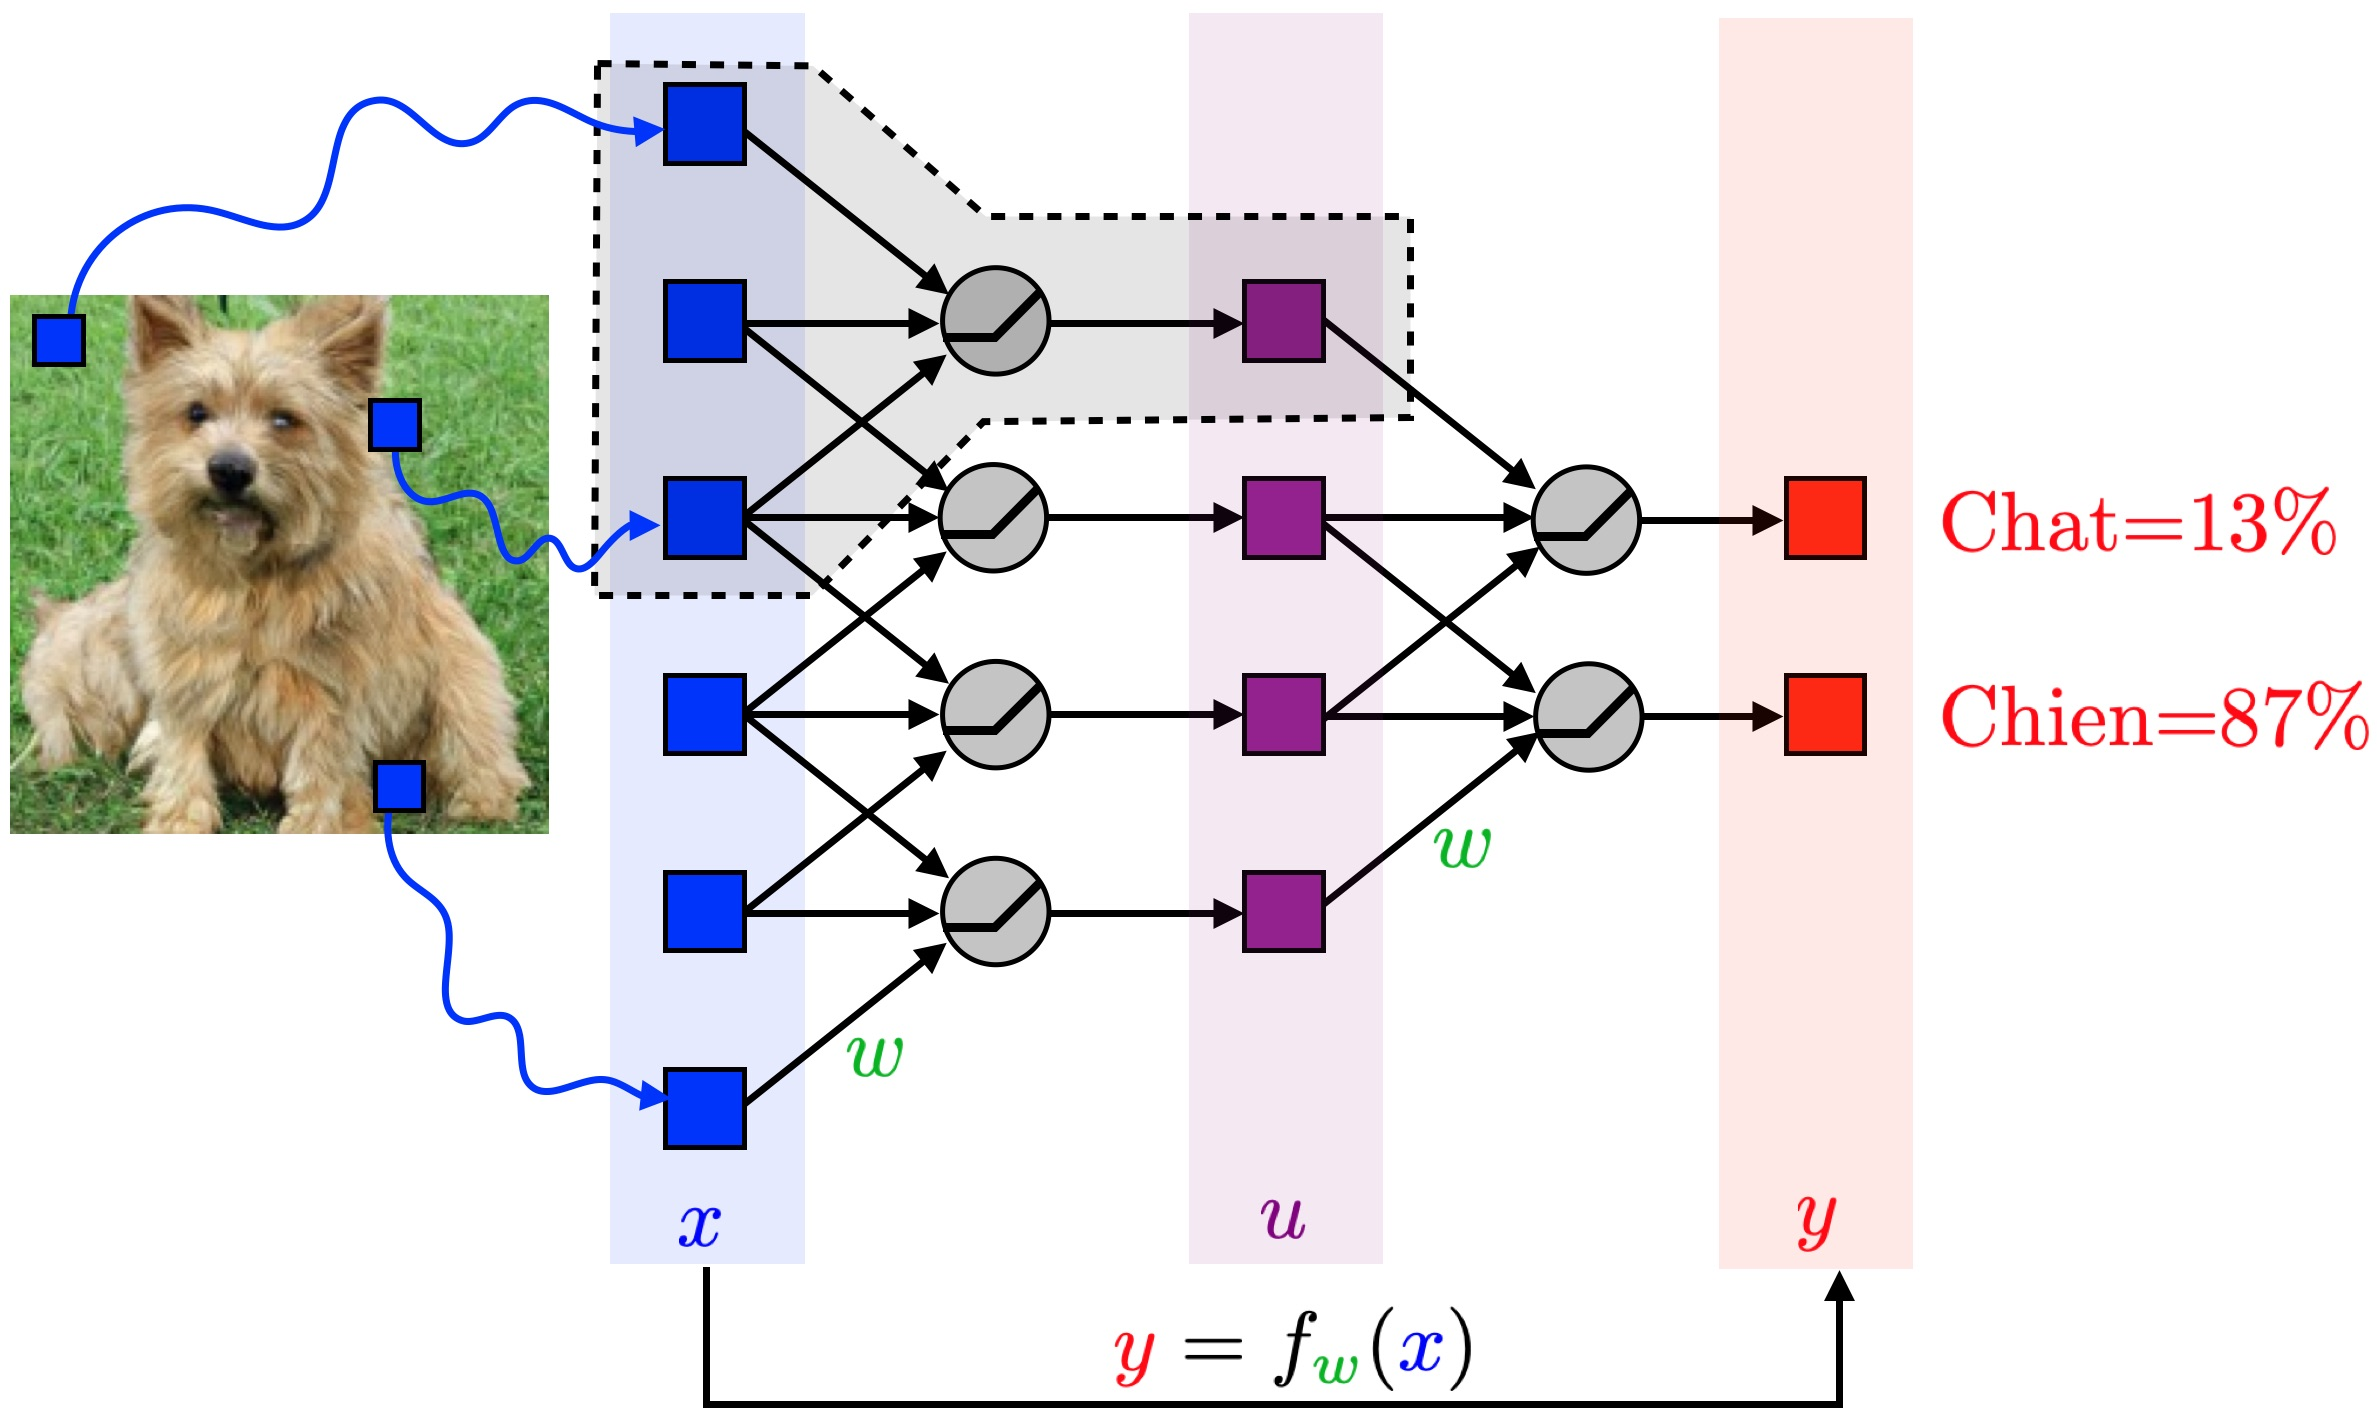
\includegraphics[width=.8\linewidth]{discriminative}
\caption{\label{fig:discriminative} Exemple d'un réseau de neurones discriminatif avec deux couches.  }
\end{figure}

La figure~\ref{fig:discriminative} détaille un exemple d'un tel réseau artificiel.
%
Ce type de neuron a été introduit en 1943 par McCulloch et Pitts~\cite{mcculloch1943logical}.
%
Pour simplifier, il est ici composé de seulement deux couches de neurones (la première couche entre ${\color{blue} x}$ et ${\color[rgb]{.5,0,.5} u}$, la deuxième entre ${\color[rgb]{.5,0,.5} u}$ et ${\color{red} y}$), mais les réseaux actuels les plus performants peuvent comporter plusieurs dizaines de couches, on dit qu'ils sont plus profonds. 
%
Dans notre exemple, les entrées ${\color{blue} x}$ sont les pixels d'une image. Une image contient typiquement des millions de pixels, et la figure n'en représente volontairement qu'un petit nombre : un réseau réaliste est très complexe. De plus, chaque pixel qui compose ${\color{blue} x}$ est en fait composé de 3 valeurs (une pour chaque couleur primaire rouge, vert et bleu). 

Le passage d'une couche (par exemple la couche ${\color{blue} x}$ des entrées) à une autre (par exemple la deuxième couche ${\color[rgb]{.5,0,.5} u}$, qui est une couche \guill{cachée} au milieu du réseau) se fait par l'intermédiaire d'un ensemble de neurones artificiels. Un neurone est représenté sur la figure~\ref{fig:neuron}. C'est le premier neurone, celui qui calcule la première valeur ${\color[rgb]{.5,0,.5} u_1}$ qui compose la couche ${\color[rgb]{.5,0,.5} u}$. Ce neurone connecte un certain nombre d'éléments de la première couche (ici trois : ${\color{blue} x_1, x_2, x_3}$, mais il peut y en avoir plus) à un seul élément de la deuxième, donc ici ${\color[rgb]{.5,0,.5} u_1}$. La formule calculée par le neurone est 
$$
	{\color[rgb]{.5,0,.5} u_1} = \max( \mygreen{w_1} \times \myblue{x_1} + \mygreen{w_2} \times \myblue{x_2} + \mygreen{w_3} \times \myblue{x_3} + \mygreen{w_4}, 0 ).
$$ 
Le neurone effectue ainsi une somme pondérée des trois entrées, avec trois poids $\mygreen{w_1},\mygreen{w_2},\mygreen{w_3}$, et on ajoute également $\mygreen{w_4}$, qui est un biais. Puis le neurone calcule le maximum entre cette somme et zero. On peut également utiliser une autre fonction que la fonction maximum, mais celle-ci est la plus populaire. Il s'agit d'une opération de seuillage. On peut la comparer aux neurones biologiques qui laissent ou non passer l'information suivant s'ils sont suffisamment excités ou pas.   
%
Ainsi, si la somme pondérée 
$\mygreen{w_1} {\color{blue} x_1} + \mygreen{w_2} {\color{blue} x_2} + \mygreen{w_3} {\color{blue} x_3} + \mygreen{w_4}$ 
est plus petite que 0, alors le neurone renvoie la valeur ${\color[rgb]{.5,0,.5} u_1}=0$, sinon il renvoie la valeur de cette somme et la place dans ${\color[rgb]{.5,0,.5} u_1}$.


\begin{figure}\centering
	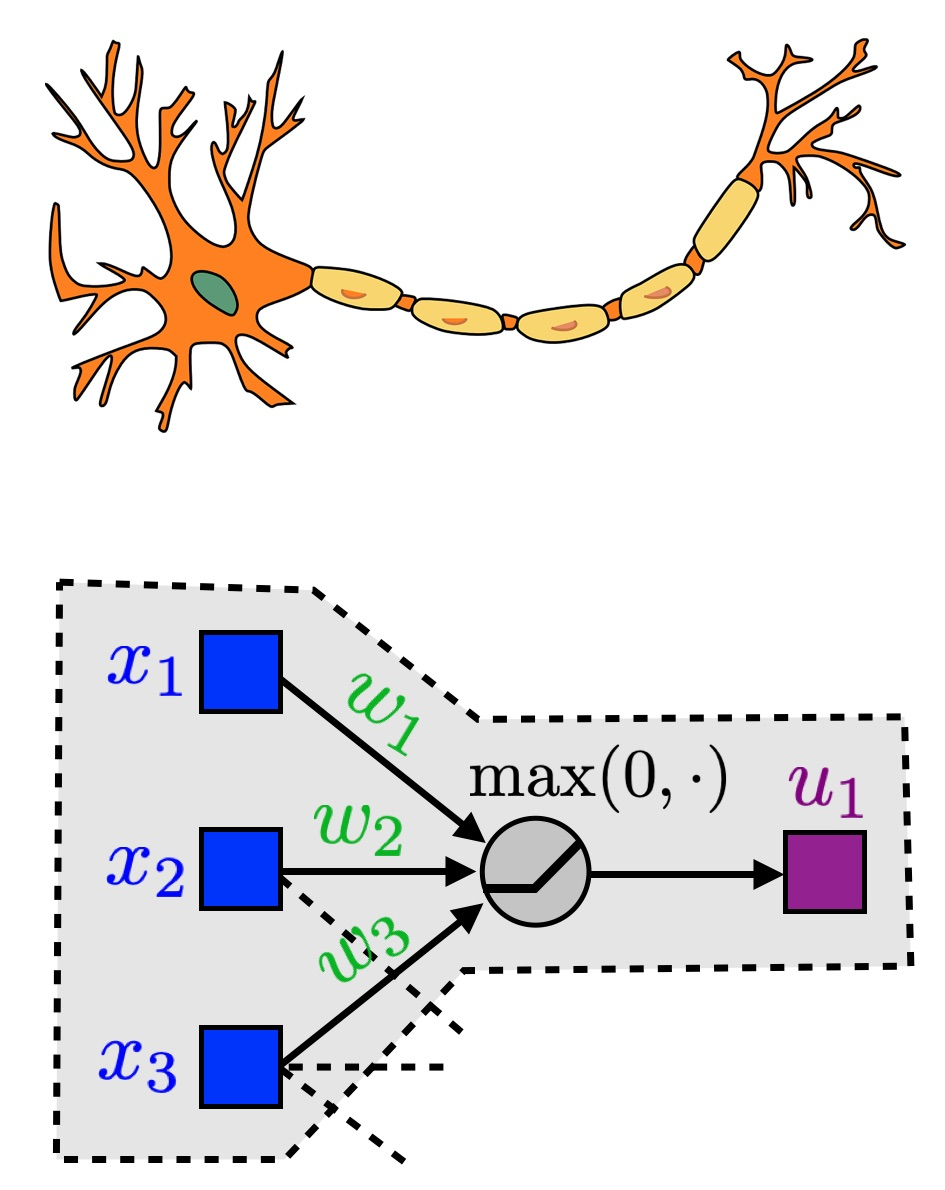
\includegraphics[width=.35\linewidth]{neuron}
\caption{\label{fig:neuron} Neurones biologique et artificiel. }
\end{figure}

De tels réseaux de neurones ont été introduits par Rosenblatt~\cite{rosenblatt1957perceptron} en 1957, qui les a appelés \guill{perceptrons}. 
% Ils ont ensuite été popularisés par le livre de Minsky et Papert~\cite{minsky1969perceptrons}. 
Les premiers perceptrons ne contenaient qu'une seule couche. 
%
De telles architectures avec une seule couche sont trop simples pour pouvoir effectuer des tâches complexes. C'est en rajoutant plusieurs couches que l'on peut calculer des fonctions plus complexes. 
%
Les réseaux de neurones profonds utilisent ainsi un très grand nombre de couches. Depuis quelques années, ces architectures ont permis d'obtenir des résultats très impressionnants pour faire de la reconnaissance d'images et de vidéos ainsi que pour la traduction automatique de textes. Ce sont ces recherches sur les réseaux profonds qui ont permises au chercheur français Yann Le Cun ainsi qu'à Geoffrey Hinton et Yoshua Bengio~\cite{lecun2015deep} d'obtenir le prix Turing en 2019. Ce prix est considéré comme étant l'équivalent du prix Nobel en informatique.  
%
Pour se familiariser avec ces réseaux multi-couches, on peut utiliser l'application interactive \url{https://playground.tensorflow.org}.

%%%%%%%%%%%%%%%%%%%%%%%%%%%%%%%%%%%%%%%%%%%%%%%%%%%%%%%%%%
\section{L'apprentissage supervisé d'un réseau de neurones}

L'entrainement d'un réseau de neurones consiste à choisir les \guill{meilleurs} poids possibles de l'ensemble des neurones qui compose un réseau (par exemple en particulier les poids $\mygreen{w_1, w_2}$ et $\mygreen{w_3}$ du neurone montré à la figure~\ref{fig:neuron}). 
%
Il faut ainsi choisir les valeurs de ces poids afin de résoudre le mieux possible la tâche étudiée, et ceci sur un ensemble de données d'apprentissage. 
%
Pour la reconnaissance d'objets dans les images, il s'agit d'un problème d'apprentissage supervisé : on dispose à la fois des images ${\color{blue} x}$ et des ${\color{red} y}$ (les probabilités de présence d'un chat et/ou d'un chien dans l'image).
%
La figure~\ref{fig:dataset} montre quelques exemples d'images utilisées pour entrainer un réseau, pour lesquelles on sait ce qu'elles contiennent (la classe des chats et la classe des chiens). 
%
Il faut donc, en amont de la phase d'apprentissage, que des humains fasse un long et fastidieux travail d'étiquetage de milliers voir de millions d'images. 


\begin{figure}\centering
	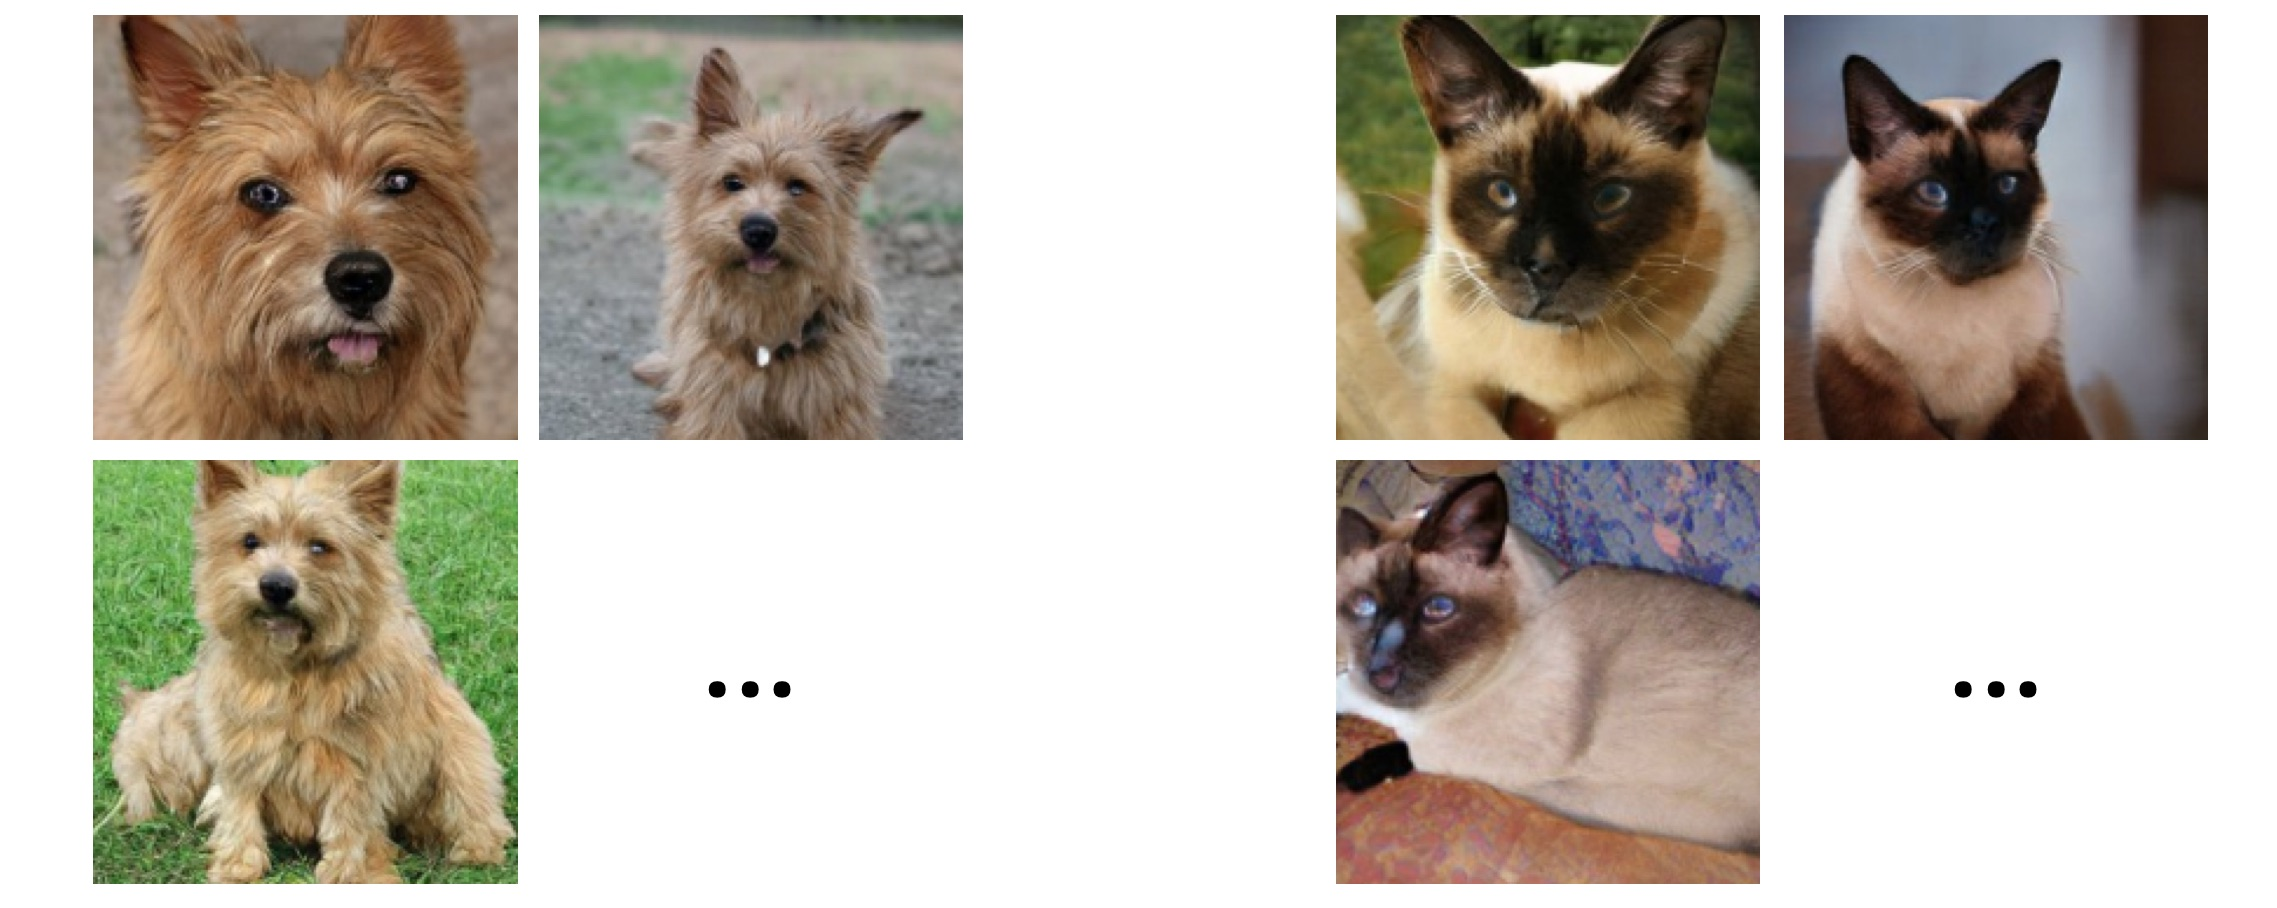
\includegraphics[width=.8\linewidth]{dataset}
\caption{\label{fig:dataset} Exemples d'images issues de la base de données ImageNet~\cite{deng2009imagenet} utilisées pour l'apprentissage. }
\end{figure}

La procédure d'entrainement consiste ainsi à modifier les poids $\mygreen{w}$ tels que pour chaque ${\color{blue}x}$, le réseau $f_{\mygreen{w}}$ prédise aussi précisément que possible le ${\color{red} y}$ associé, c'est-à-dire que l'on souhaite à la fin de l'entrainement que ${\color{red} y} \approx f_{\mygreen{w}}({\color{blue} x})$. 
%
Un choix simple est de minimiser la somme $E(\mygreen{w})$ des carrés des erreurs, ce qu'on écrit mathématiquement comme 
$$
	\min_{\mygreen{w}} E(\mygreen{w}) = \sum_{({\color{blue} x},{\color{red} y})} (f_{\mygreen{w}}({\color{blue} x}) - {\color{red} y})^2.
$$
%
Ceci correspond à un problème d'optimisation, car il faut trouver un jeu de paramètres qui optimise une certaine quantité d'intérêt. 
%
C'est un problème difficile, car il y a beaucoup de paramètres, et ces paramètres, surtout ceux des couches cachées, influencent de façon très subtile le résultat.
%
Heureusement, il existe des méthodes mathématiques et algorithmiques performantes pour résoudre de façon satisfaisante ce type de problème d'optimisation. Elles ne sont pas encore totalement comprises sur le plan théorique et c'est un domaine de recherche en pleine explosion.
%
Ces méthodes d'optimisation modifient les poids $\mygreen{w}$ du réseau pour l'améliorer et diminuer l'erreur d'entrainement $E(\mygreen{w})$. La règle mathématique pour décider de la stratégie de mise à jour des poids s'appelle la rétro-propagation~\cite{rumelhart1986learning} et est une merveille d'ingéniosité, c'est un cas particulier d'une méthode mathématique et algorithmique qui s'appelle la différentiation automatique à l'envers~\cite{linnainmaa1976taylor}.

Ces techniques d'apprentissage supervisé datent pour l'essentiel des année 1980. Mais c'est seulement en 2012 qu'un papier de Krizhevsky,  Sutskever et Hinton~\cite{krizhevsky2012imagenet} crée un coup de tonnerre en montrant que les réseaux profonds permettent de résoudre efficacement des problème de reconnaissance d'images. 
%
Cette révolution a été possible grâce à la combinaison de trois ingrédients: des nouvelles bases de données beaucoup plus grandes qu'auparavant~\cite{deng2009imagenet} ;  des grosses puissances de calcul grâce aux processeurs graphiques (les \guill{GPUs} , qui étaient auparavant cantonnés aux jeux vidéo) ;  l'introduction de plusieurs techniques d'optimisation qui stabilisent l'apprentissage~\cite{srivastava2014dropout}. 


%%%%%%%%%%%%%%%%%%%%%%%%%%%%%%%%%%%%%%%%%%%%%%%%%%%%%%%%%%
\section{L'efficacité des réseaux de neurones}

George Cybenko a démontré en 1989~\cite{cybenko1989approximation} qu'un réseau de neurones $f_{\mygreen{w}}$ avec deux couches peut approcher aussi précisément que l'on veut n'importe quelle fonction continue $f^\star$ (donc en quelque sorte résoudre n'importe quelle tâche, représentée par la fonction $f^\star$ inconnue, qui serait capable de reconnaitre des objets dans n'importe quelle image) pour peu que la taille de la couche interne ${\color[rgb]{.5,0,.5} u}$ (donc le nombre de neurones) soit arbitrairement grande.
%
Ce n'est pas pour autant qu'un tel réseau $f_{\mygreen{w}}$ avec seulement deux couches marche bien en pratique. Pour appliquer le théorème de Cybenko, il faut pouvoir disposer d'un nombre de donnée d'apprentissage potentiellement infini, ce qui est très loin d'être le cas en pratique.
%
Le but final de l'apprentissage n'est pas de minimiser l'erreur d'apprentissage $E(\mygreen{w})$, mais de pouvoir prédire aussi précisément que possible sur des nouvelles données. Si l'on dispose de peu de données, on risque de ne pas pouvoir apprendre assez précisément, et donc de faire des mauvaises prédictions : la fonction $f_{\mygreen{w}}$ sera en réalité très loin de la fonction $f^\star$ idéale que l'on voudrait apprendre si on avait une infinité d'exemples.  

Afin d'effectuer les meilleures prédictions possibles avec un nombre limité de données d'entrainement, on cherche donc les architectures de réseaux les plus adaptées, qui peuvent capter efficacement l'information présente dans les données. 
%
Les réseaux de neurones profonds (avec de nombreuses couches) mais avec relativement peu de connexions entre les couches se sont avérés très efficaces sur les données très \guill{structurées} comme les textes, les sons et les images. 
%
Par exemple, pour une image, les pixels ont des relations de voisinage, et on peut imposer des connexions spécifiques (une architecture) et ne pas connecter un neurone avec tous les autres mais seulement avec ses voisins (sinon il y aurait trop de connexions). De plus, on peut imposer que les poids associés à un neurone soit les mêmes que ceux associés à un autre neurone. On appelle ce type de réseaux les réseaux convolutifs~\cite{lecun1998gradient}. 
%
Pour l'instant, il n'y a pas d'analyse mathématique qui explique cette efficacité des réseaux convolutifs profonds. Il y a donc besoin de nouvelles avancées mathématiques pour comprendre les comportements et les limitations de ces réseaux profonds. 



%%%%%%%%%%%%%%%%%%%%%%%%%%%%%%%%%%%%%%%
\chapter{Les réseaux génératifs}
In the previous article, we saw how to train neural networks in a supervised manner. This makes it possible to effectively solve classification problems, for example image recognition.
%
What is perhaps even more surprising is that these neural networks are also used in an unsupervised manner in order to automatically generate \guill{virtual} texts or images, which are often called \guill{deep fakes}.
%
In this second article, I will draw a link between the learning of generative neural networks and the theory of optimal transport. This problem was framed by Gaspard Monge in the 18$^{\text{th}}$ century, then it was reformulated by Leonid Kantorovitch in the middle of 20$^{\text{th}}$ century. It has now become a tool of choice to tackle important problems in data science.
% !TEX root = ../NeuralNetworksEN.tex


%%%%%%%%%%%%%%%%%%%%%%%%%%%%%%%%%%%%%%%%%%%%%%%%%%%%%%%%%%

\section{Generative neural networks}

Instead of using neural networks to analyze images, the paper~\cite{goodfellow2014generative} has shown in 2014 that they can be used \guill{backwards} to generate images.
%
These generative neural networks, for example, find applications for special effects, video games and artistic creation.
%
Similar questions and methods can be found in the training of autonomous cars and to solve strategy games.
%
Figure~\ref{fig:generative} shows the structure of such a network $g_{\mygreen{w}}$, which depends on weights $\mygreen{w}$. The layers somehow play mirror roles compared to the architecture of the discriminating neural networks exposed in the previous article.
%
From an entry ${\color{red} y}$ composed of a small number of values, which are typically drawn randomly, one generates an image ${\color{blue} x} = g_{\mygreen{ w}}({\color{red} y})$.

\begin{figure}\centering
	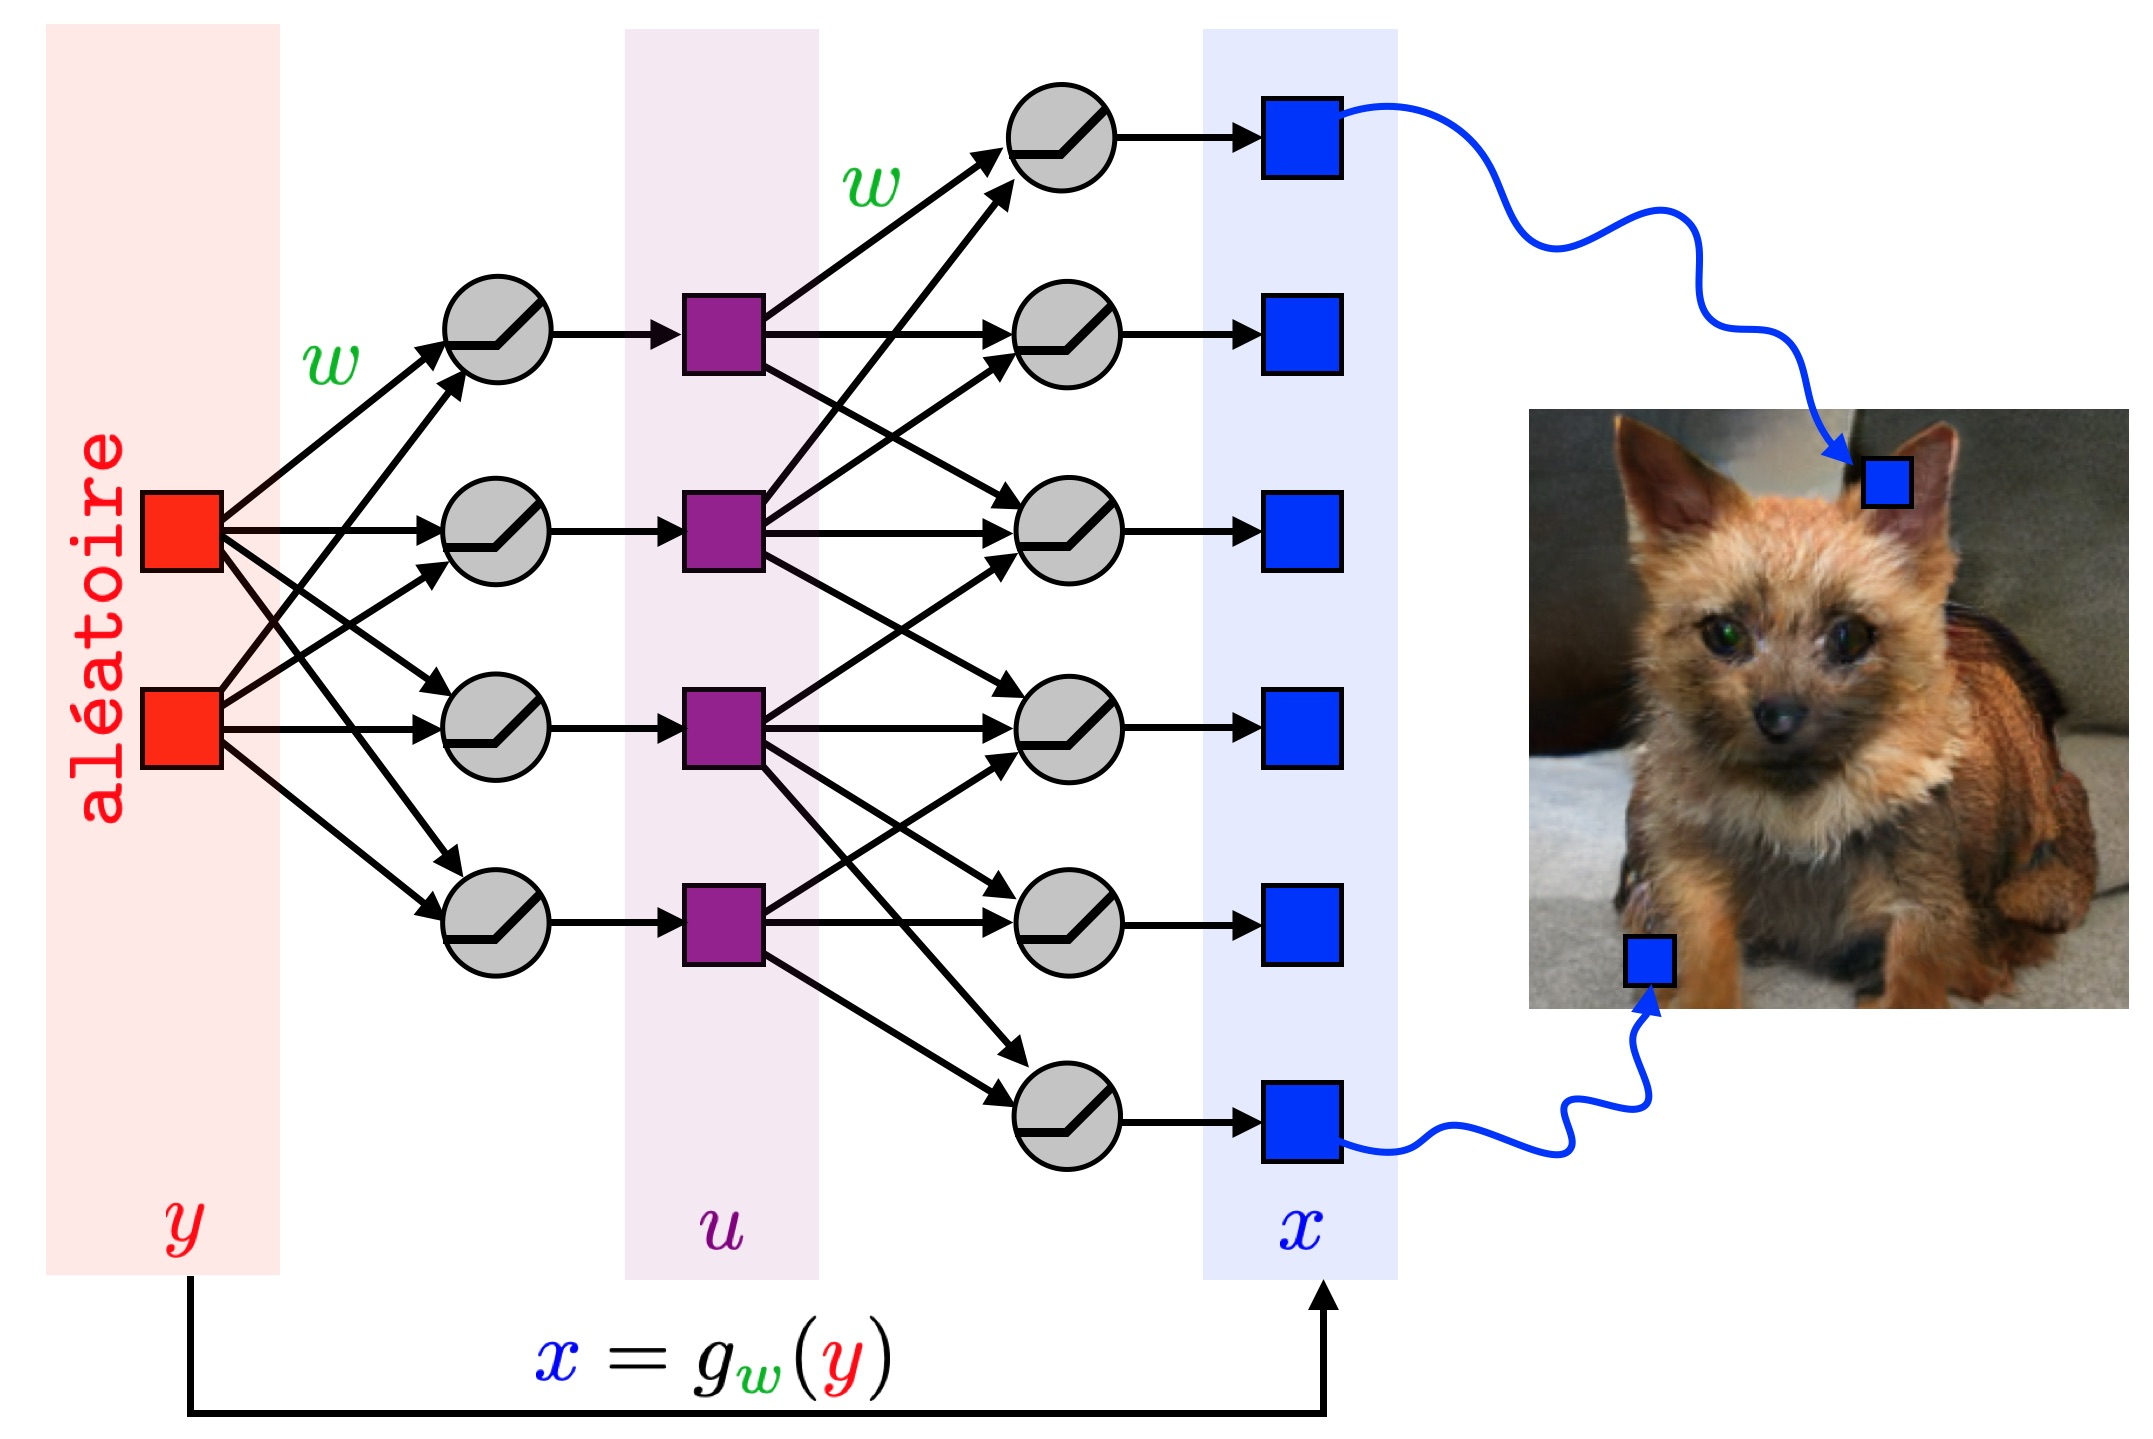
\includegraphics[width=.8\linewidth]{generative}
\caption{\label{fig:generative} Example of a simplified generative neural network (a network for generating such complex images has more layers).  }
\end{figure}

The problem of training such networks is unsupervised: there is only a large number of training images, without indication of what they contain.
%
There is no longer any need for human intervention to indicate to the network the content of the images which it must recognize.
Data collection is thus simpler than for training discriminatory networks. In addition, this principle of unsupervised learning is close to the way children learn, mainly by observing and manipulating the world around them.
%
The goal is then to select the weights $\mygreen{w}$ of the neurons of the network $g_\mygreen{w}$ so that the random images generated (the \guill{fake} images) resemble as closely as possible the images of the training set.

%%%%%%%%%%%%%%%%%%%%%%%%%%%%%%%%%%%%%%%%%%%%%%%%%%%%%%%%%%
\section{Unsupervised learning of generative networks}
\label{sec-app-gen}

The goal of generative neural networks is not to solve a task such as recognizing objects in images.
%
In order to train the weights $\mygreen{w}$ of the network, the problem must be formalized mathematically. This involves generating a set of \guill{virtual} images (the false ones) that look like real images in a database. It is not simply that a generated image looks like a real image, it is necessary to match the two sets of images. For example, if in the database there are half images of dogs and half images of cats, the network must also generate half of dogs and half of cats.

We will write $\{\mylblue{z_1, z_2, \ldots, z_n}\}$ the set of $n$ images in the database. The number $n$ of images is very large, of the order of several thousand or millions. Given a generative neural network $g_{\mygreen{w}}$, which is parameterized by its weights $\mygreen{w}$, we note $\{\myblue{x_1, x_2, \ldots, x_n} \}$ a set of $n$ \guill{false} images randomly generated by the network. To generate the first false image $\mylblue{x_1}$, this means that we randomly draw the input values ${\color{red} y_1}$ and apply the network to these inputs, to obtain the virtual image $\mylblue{x_1} = g_{\mygreen{w}}({\color{red} y_1})$. We then do the same thing with $\mylblue{x_2} = g_{\mygreen{w}} ({\color{red} y_2})$ and so on.

The goal of unsupervised learning is therefore to find weights $\mygreen{w}$ so that the set of false images $\{\myblue{x_1, \ldots, x_n} \}$ is as close as possible to the set of images $\{\mylblue{z_1, \ldots, z_n}\}$ of the database. The optimization problem is written thus
\eq{
	\umin{\mygreen{w}} \text{Distance}( 
		\{\myblue{x_1,\ldots,x_n} \}, 
		\{\mylblue{z_1,\ldots,z_n}\}  ).
}
It should here be remembered that the images generated $\{\myblue{x_1, \ldots, x_n} \}$ depend on the network $g_{\mygreen{w}}$ and therefore on the weights $\mygreen{w}$. We can reformulate the previous problem as
\eq{
	\umin{\mygreen{w}} \text{Distance}( 
		\{g_{\mygreen{w}}({\color{red}y_1}),\ldots, g_{\mygreen{w}}({\color{red}y_n})\}, 
		\{\mylblue{z_1,\ldots,z_n}\}  ).
}
%
The mathematical question that arises is therefore to define a notion of distance between two sets of points. There are many ways to do this, and we will explain one that is well suited to this learning problem.
%
It exploits the theory of optimal transport.


%%%%%%%%%%%%%%%%%%%%%%%%%%%%%%%%%%%%%%%%%%%%%%%%%%%%%%%%%%
\section{Monge's optimal transport}
\label{sec-ot}

The optimal transport problem is formulated by Gaspard Monge~\cite{Monge1781} in 1781, for military applications.
%
The question asked is to determine the most economical way to transfer objects from a set of sources $\{\myblue{x_1, \ldots, x_n}\}$ to a set of destinations $\{\mylblue{z_1, \ldots, z_n}\}$. For Monge, it is a matter of transferring soil from cuttings to create embankments. But this question finds a multitude of applications.
%
For the problem of training generative networks, the sources are the false images generated by the network and the destinations are the images of the database.

\newcommand{\perm}[1]{s_{#1}}

It is thus necessary to link each source, for example $\myblue{x_1}$ to a single destination point, which we will note $\mylblue{z_{\perm{1}}}$, where $\perm{1}$ is an integer between $1$ and $n$. Similarly, ${\color{blue} x_2}$ is linked to $\mylblue{z_{\perm{2}}}$ and so on. For example, in figure~\ref{fig:otmonge}, we link $\myblue{x_2}$ to $\mylblue{z_5}$, which means that $\perm{\myblue{2}} = \mylblue{5}$.
%
Each of the $n$ destinations must also be supplied by a source. This means for example that ${\color{blue} x_1}$ and ${\color{blue} x_2}$ cannot be linked to the same destination, all the sources must be linked to different destinations. This means that $\{\perm{1}, \ldots, \perm{n}\}$ must be a permutation of the first $n$ integer numbers.
%
For example, on the figure~\ref{fig:otmonge}, on a simple example with $n=6$ elements, we have chosen on the left the permutation
\eq{
	(\perm{\myblue{1}}=\mylblue{1},
	\perm{\myblue{2}}=\mylblue{5},
	\perm{\myblue{3}}=\mylblue{4},
	\perm{\myblue{4}}=\mylblue{6},
	\perm{\myblue{5}}=\mylblue{3},
	\perm{\myblue{6}}=\mylblue{2}).
}
%
Monge's problem then consists in finding the permutation which minimizes the sum of the transport costs. Monge decided that the cost of transportation between a source $\myblue{x}$ and a destination $\mylblue{z}$ is equal to the Euclidean distance $\norm {\myblue{x} - \mylblue{z}}$ between the two points, but one can choose another cost: for example a travelling time or the price required for gasoline if using trucks, etc. We have to solve the problem
\eq{
	\umin{\text{permutation } s} 
		\norm{\myblue{x_1} - \mylblue{z_{\perm{1}}}} + 
		\norm{\myblue{x_2} - \mylblue{z_{\perm{2}}}} + 
		\ldots + 
		\norm{\myblue{x_n} - \mylblue{z_{\perm{n}}}}.
}
Once we have calculated an optimal permutation $s^\star = (\perm{1}^\star, \ldots, \perm{n}^\star)$ (i.e. which is solution of the previous problem), we define the distance between the sets of points as the value of the total transport cost
\eq{
	\text{Distance}( 
		\{\myblue{x_1,\ldots,x_n} \}, 
		\{\mylblue{z_1,\ldots,z_n}\}  ) 
	\eqdef 
		\norm{\myblue{x_1} - \mylblue{z_{\perm{1}^\star}}} + 
		\norm{\myblue{x_2} - \mylblue{z_{\perm{2}^\star}}} + 
		\ldots + 
		\norm{\myblue{x_n} - \mylblue{z_{\perm{n}^\star}}}.
}

\begin{figure}\centering
	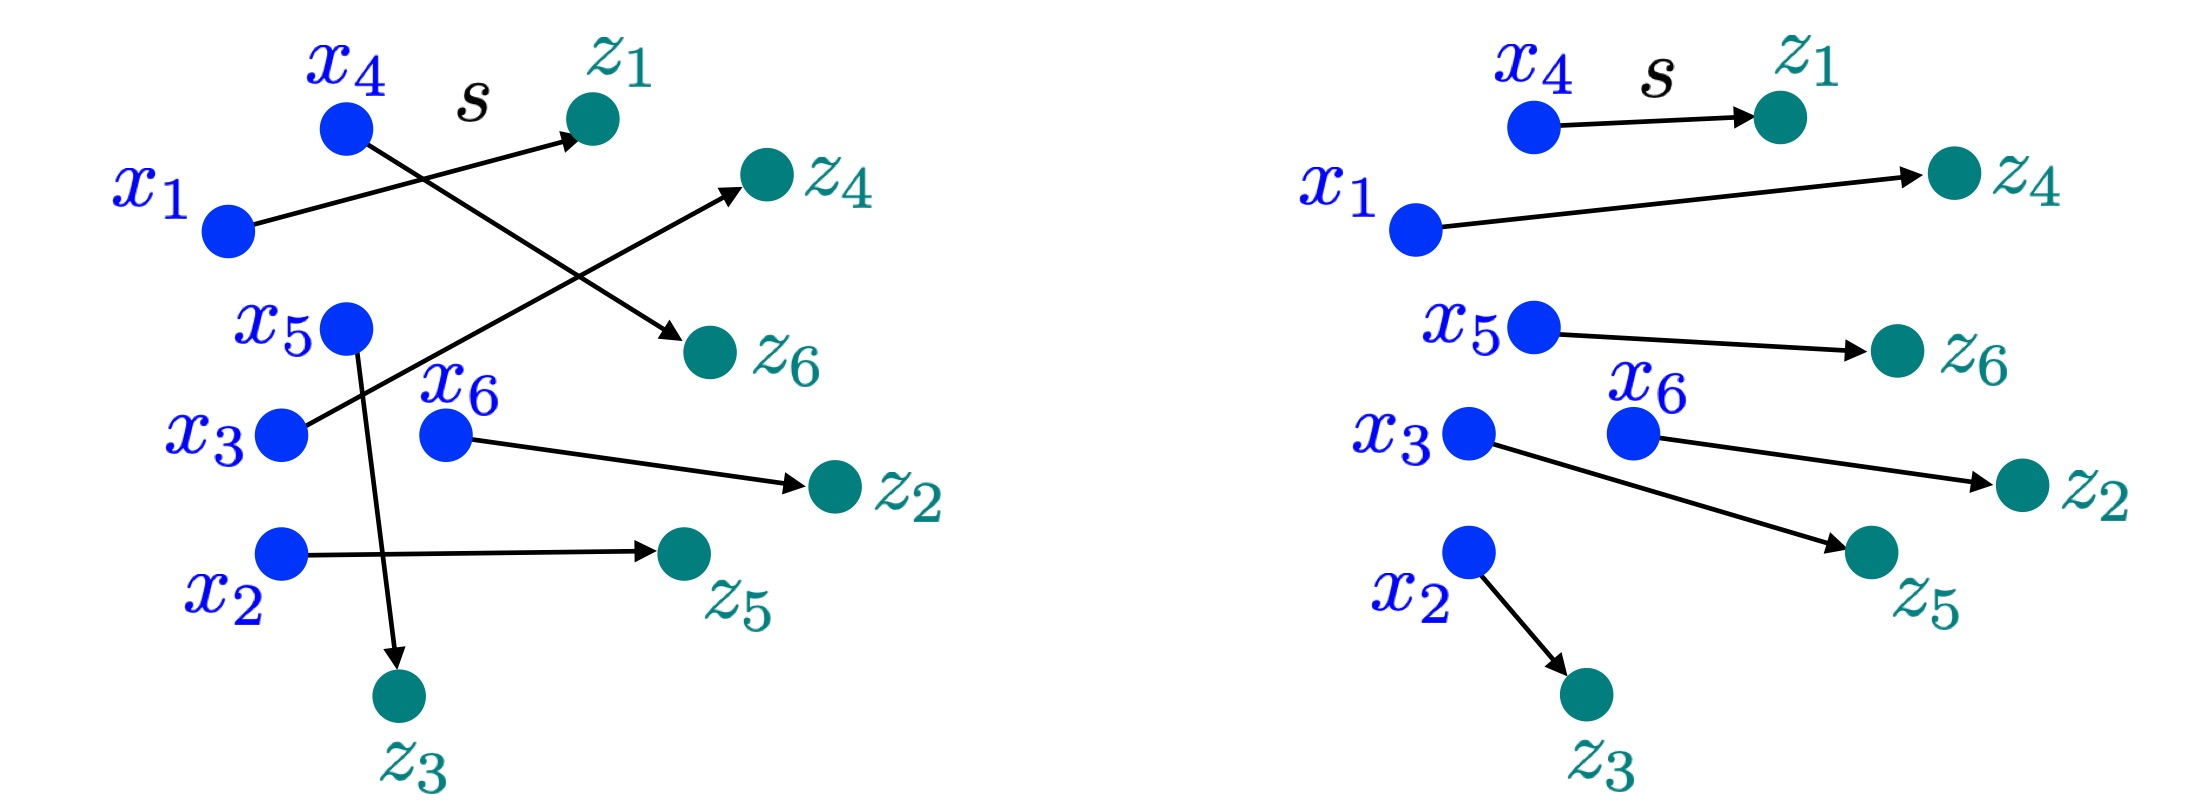
\includegraphics[width=.8\linewidth]{otmonge.jpg}
\caption{\label{fig:otmonge} Example on the left of a non-optimal permutation $s$ and on the right of the optimal permutation, in the case of $6$ points in dimension 2.  }
\end{figure}

The difficulty in calculating this distance is that the total number of permutations to be tested is very large. Indeed, for the choice of $\perm{1}$ there are $n$ possibilities, for that of $\perm{2}$ there is $n-1$ (since the value of $\perm{1}$ is taken), for $\perm{2}$ there is $n-2$, etc. So the total number of permutations is $n!$, The factorial of the number $n$, which is defined as
\eq{
	n! = n \times (n-1) \times (n-2) \times \ldots \times 2 \times 1.
}
For $n=6$ as in the figure~\ref{fig:otmonge}, there is therefore
\eq{
	6! = 6 \times 5 \times 4 \times 3 \times 2 \times 1 = 720 \text{ possible permutations.}
}
In this simple case, we can test them all and choose the best one, which is, as shown on the right of the figure~\ref{fig:otmonge},
\eq{
	(\perm{\myblue{1}}=\mylblue{4},
	\perm{\myblue{2}}=\mylblue{3},
	\perm{\myblue{3}}=\mylblue{5},
	\perm{\myblue{4}}=\mylblue{1},
	\perm{\myblue{5}}=\mylblue{6},
	\perm{\myblue{6}}=\mylblue{2}).
}
The difficulty is that for $n = 70$, there are more than $10^{100}$ possibilities, which is to be compared to the $10^{79}$ atoms in the universe \ldots And to train neural networks, $n$ is even much bigger!
%
It was therefore necessary to wait for several mathematical and algorithmic revolutions before being able to obtain a method enabling this problem to be resolved.


%%%%%%%%%%%%%%%%%%%%%%%%%%%%%%%%%%%%%%%%%%%%%%%%%%%%%%%%%%
\section{The optimal transport of Kantorovitch}
\label{sec-kanto}

Monge has noticed that the solutions to his problem have very specific structures. For example, we can observe in the figure~\ref{fig:otmonge}, on the right, that the optimal paths do not cross, and Monge proved it in his article~\cite{Monge1781}. But this is not enough to solve the problem, because there are still a lot of paths without crossing. It took over 200 years to figure out how to get more information about the solutions in order to calculate them efficiently.
%
It was Leonid Kantorovitch who found, in 1942~\cite{Kantorovich42}, a new formulation of the problem of optimal transport. He allowed each source to be divided into several parts, for example two equal parts with a weighting of 1/2 each. This division of production is interesting because it simplifies the optimization problem. It is also natural for the problem studied by Kantorovitch who was trying to model and plan production in economics. He won the Nobel Prize in economics for this idea.
%
Together with these pioneering works by Kantorovitch, George Dantzig introduced in 1947 the simplex algorithm~\cite{dantzig1990origins}, which makes it possible to efficiently solve large scale transport problems. Its numerical complexity to solve an optimal transport problem between $n$ points is of the order of $n^3 = n \times n \times n$, which is much lower than $n! = n  \times (n-1) \times \ldots \times 2 \times 1$. It is at the heart of a very large number of industrial systems which must optimize the adequacy between means of production and consumption. And we can also use it to train generative neural networks! One can look at~\cite{PeyreCuturi} for more details on the optimal transport theory, efficient algorithms and its applications to data science.


%%%%%%%%%%%%%%%%%%%%%%%%%%%%%%%%%%%%%%%%%%%%%%%%%%%%%%%%%%
\section{Adversarial networks}

One difficulty in applying optimal transport to generate generative networks is that it is necessary to choose the transport cost between two images.
%
We could calculate the Euclidean distance between the pixels of the images, but this does not work well, because it does not take into account the geometry of the objects present in the images.
%
A very successful idea was introduced in 2014 by Ian Goodfellow and his collaborators~\cite{goodfellow2014generative}. It can be interpreted as using a second neural network to determine this transport cost~\cite{martin2017wasserstein}.
%
This second network $f$, called adversary network, plays a discriminative role. While the goal of the generator $g$ is to generate  fake images which looks real, the goal of $f$ is, on the contrary, to do its best to recognize true and false images. These two networks are jointly trained, this is why one speaks of adversarial networks.
%
The training of these two networks corresponds to what is called a zero-sum game, introduced by John Von Neumann in 1944~\cite{morgenstern1953theory} and then generalized by John Nash in 1950~\cite{nash1950equilibrium}, which just like Kantorovitch obtained the Nobel Prize in economics.

These recent advances~\cite{goodfellow2014generative} have made it possible to obtain excellent results for image generation.
%
The figure~\ref{fig:deepfake} shows results obtained with the method explained in~\cite{brock2018large} and its use to calculate \guill{paths} of images between dogs and cats.

\begin{figure}\centering
	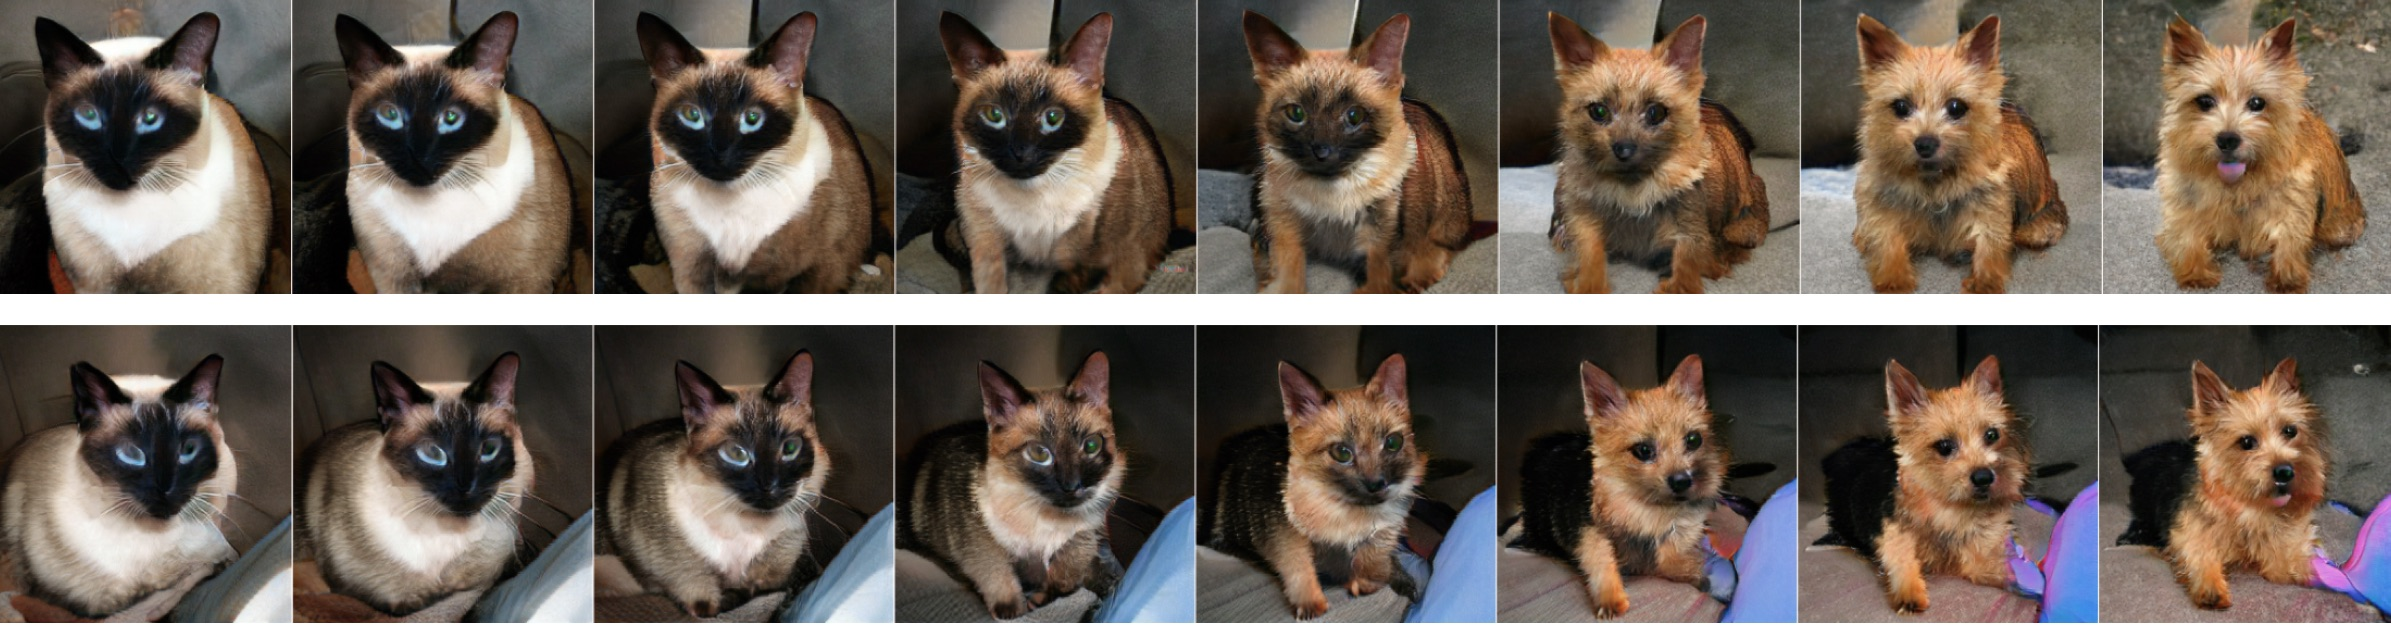
\includegraphics[width=.95\linewidth]{deepfake}
\caption{\label{fig:deepfake} Two examples of \guill{deep fakes} which are virtual images interpolating between cats and dogs. }
\end{figure}




\section*{Remerciements}

Je remercie Gwenn Guichaoua pour sa relecture attentive, ainsi que Sébastien Racanière et Vincent Barra pour leurs corrections.

\bibliographystyle{plain}
\bibliography{biblio-nn}

\end{document}

